\documentclass{article}
	\def\lettertitle{Author Response to Reviewer-ABCD of Paper-5736:}
	\def\papertitle{Adaptive Variational Nonlinear Chirp Mode Decomposition}
	\def\authors{Hao Liang, Xinghao Ding, Andreas Jakobsson, Xiaotong Tu*, Yue Huang}
	\def\journal{Submitted to 2022 IEEE International Conference on Acoustics, Speech and Signal Processing}

\usepackage[includeheadfoot,top=5mm, bottom=5mm, footskip=2.5cm]{geometry}
\usepackage[T1]{fontenc}
\usepackage{times}
\usepackage{amssymb,amsmath}
\usepackage{microtype}                         
\usepackage[utf8]{inputenc}
\usepackage{graphicx}
\usepackage[hidelinks]{hyperref} 
\usepackage{soul} % Highlight using \hl{}
\usepackage{adjustbox} % center large tables across textwidth by surrounding tabular with \begin{adjustbox}{center}
\renewcommand{\arraystretch}{1.2} % enlarge spacing between rows
\usepackage{caption} 
\captionsetup[table]{skip=10pt} % enlarge spacing between caption and table
\usepackage{titlesec}

\usepackage{cite}
\usepackage{graphicx}
\graphicspath{{./figures/}}
\usepackage{subfigure}

\titleformat{\section}{\normalfont\large}{\makebox[0pt][r]{\bf \thesection.\hspace{4mm}}}{0em}{\bfseries}
%\titleformat{\subsection}{\normalfont}{\makebox[0pt][r]{\bf \thesubsection.\hspace{4mm}}}{0em}{\bfseries}
%\titlespacing{\subsection}{0em}{1em}{-0.3em} % left before after
\setlength{\parskip}{0.6\baselineskip}%
\setlength{\parindent}{0pt}%
\usepackage{framed}
\let\oldquote=\quote
\let\endoldquote=\endquote
\renewenvironment{quote}{\begin{fquote}\advance\leftmargini -2.4em\begin{oldquote}}{\end{oldquote}\end{fquote}}
\usepackage{xcolor}
\newenvironment{fquote}
  {\def\FrameCommand{
	\fboxsep=0.6em % box to text padding
	\fcolorbox{black}{white}}%
    \MakeFramed {\advance\hsize-2\width \FrameRestore}
    \begin{minipage}{\linewidth}
  }
  {\end{minipage}\endMakeFramed}
\let\oldtabular=\tabular
\let\endoldtabular=\endtabular
\renewenvironment{tabular}[1]{\begin{adjustbox}{center}\begin{oldtabular}{#1}}{\end{oldtabular}\end{adjustbox}}

\usepackage{suffix}
\long\def\RC#1\par{\makebox[0pt][r]{\bf \textit{RC:}\hspace{8pt}}\textbf{\textit{#1}}\par} %\RC
\WithSuffix\long\def\RC*#1\par{\textbf{\textit{#1}}\par} %\RC*
\long\def\AR#1\par{\makebox[0pt][r]{\textit{AR:}\hspace{10pt}}\textit{#1}\par} %\AR
\WithSuffix\long\def\AR*#1\par{\textit{#1}\par} %\AR*



%%%
%DIF PREAMBLE EXTENSION ADDED BY LATEXDIFF
%DIF UNDERLINE PREAMBLE %DIF PREAMBLE
\RequirePackage[normalem]{ulem} %DIF PREAMBLE
\RequirePackage{color}\definecolor{RED}{rgb}{1,0,0}\definecolor{BLUE}{rgb}{0,0,1} %DIF PREAMBLE
\providecommand{\DIFadd}[1]{{\protect\color{blue}\uwave{#1}}} %DIF PREAMBLE
\providecommand{\DIFdel}[1]{{\protect\color{red}\sout{#1}}}                      %DIF PREAMBLE
%DIF SAFE PREAMBLE %DIF PREAMBLE
\providecommand{\DIFaddbegin}{} %DIF PREAMBLE
\providecommand{\DIFaddend}{} %DIF PREAMBLE
\providecommand{\DIFdelbegin}{} %DIF PREAMBLE
\providecommand{\DIFdelend}{} %DIF PREAMBLE
%DIF FLOATSAFE PREAMBLE %DIF PREAMBLE
\providecommand{\DIFaddFL}[1]{\DIFadd{#1}} %DIF PREAMBLE
\providecommand{\DIFdelFL}[1]{\DIFdel{#1}} %DIF PREAMBLE
\providecommand{\DIFaddbeginFL}{} %DIF PREAMBLE
\providecommand{\DIFaddendFL}{} %DIF PREAMBLE
\providecommand{\DIFdelbeginFL}{} %DIF PREAMBLE
\providecommand{\DIFdelendFL}{} %DIF PREAMBLE
%DIF END PREAMBLE EXTENSION ADDED BY LATEXDIFF

\thispagestyle{empty} %Delete page number

\begin{document}
	
% Make titl
{\Large\bf \lettertitle}\\[1em]
{\LARGE \papertitle}\\[1em]
{\authors}\\
{\it \journal}\\
\hrule

\hfill  {\bfseries \textit{RC:}} \textbf{\textit{Reviewer Comment}},\(\quad\) \textit{AR:} \emph{Author Response}, \(\quad\square\): \textit{Manuscript Text}  % Legend

%\section{Importance/Relevance to ICASSP 2022}

% \section{Novelty/Originality}

\section{Experimental Validation}
\RC \rm \bf Perhaps an enlargement of the relevant parts of the graph would be useful.

\AR \rm Ok, I changed this. Please see Fig.\ref{fig1} for details.
\begin{figure}[h] 
	\centering
	\subfigure[]{
		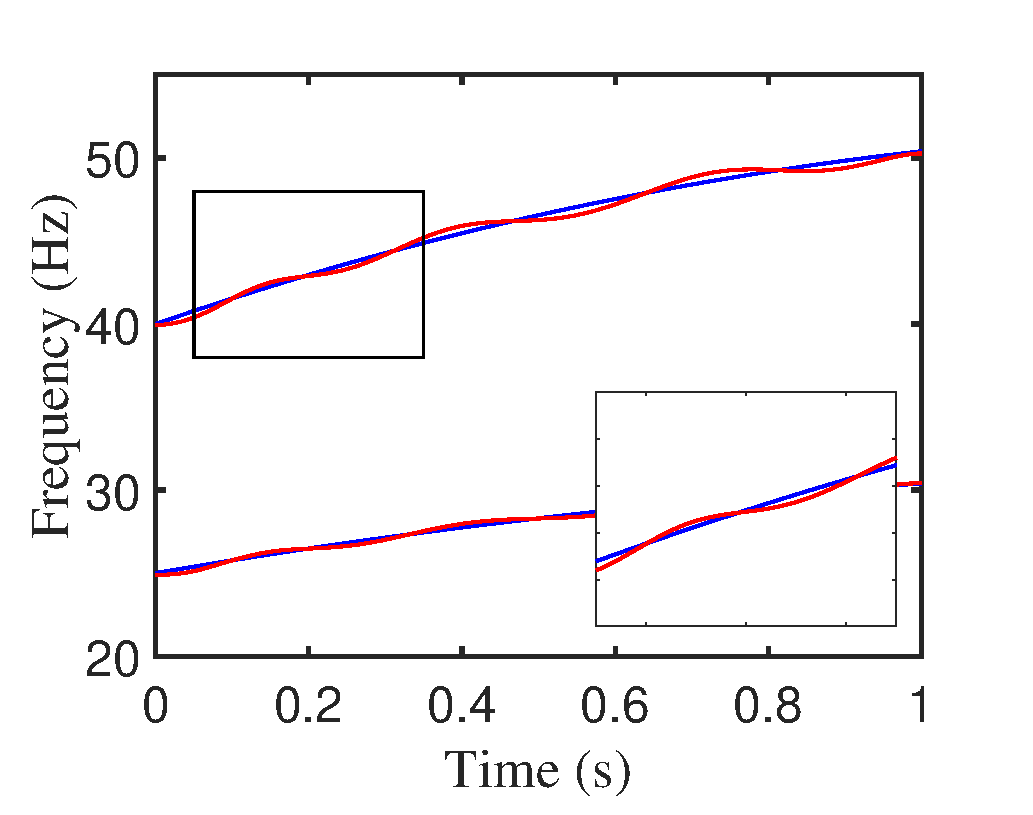
\includegraphics [width=4.5cm]{VNCMD}}
	\subfigure[]{		
		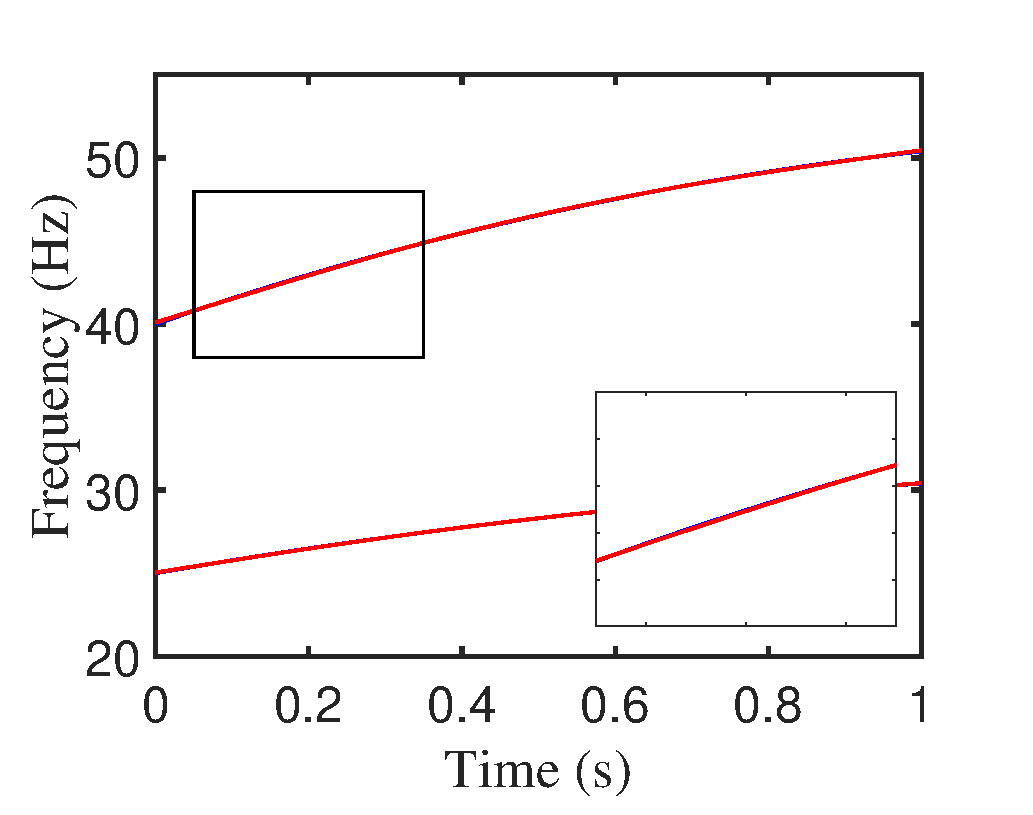
\includegraphics [width=4.5cm]{AVNCMD}}
	\caption{The estimated IFs by different algorithms (blue: true; red: estimated): (a) VNCMD, (b) AVNCMD.}
	\label{fig1}
\end{figure}

\section{Technical Correctness}
\RC \rm \bf There are some minor errors: in Equation (\ref{eq1}), notation $u_i^{k+1}$ is from \cite{chen2017nonlinear} and does not follow the paper's adopted notation.

\AR \rm Ok, I corrected this:

\begin{quote}
	The arctangent demodulation technique may be introduced to update the IF increment, i.e.,
	\begin{equation}
		\label{eq1}
		\small
		\Delta f_{k}^{(i)}(t) = \frac{v_{k}^{(i)}(t) \cdot\left(u_{k}^{(i)}(t)\right)^{\prime}-\DIFdelbegin \DIFdel{u_{i}^{k+1}(t)}\DIFdelend \DIFaddbegin \DIFadd{u_{k}^{(i)}(t)}\DIFaddend \cdot\left(v_{k}^{(i)}(t)\right)^{\prime}}{2 \pi\left[\left(u_{k}^{(i)}(t)\right)^{2}+\left(v_{k}^{(i)}(t)\right)^{2}\right]}.
	\end{equation}
\end{quote}

\AR* \noindent \rm Great, you're so careful.

\hl{\large \bf Any more questions?}
%\section{Clarity of Presentation}
	
%\section{Reference to Prior Work}


%\section{Additional comments to author(s)}

\bibliographystyle{unsrt}
\bibliography{refs}
	
\end{document}